\section{Fiche de l'Indonésie}

%\begin{multicols}{2}

%\hspace*{-0.65cm}
%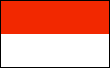
\includegraphics[width=4.8cm]{articles/Fiche-de-l-indonesie/drapeauindonesie.png}
%Drapeau de l'Indonésie.

\textbf{\textsc{Situation}}

\textbf{Présentation générale}

En Asie du Sud-Est, entre océan Indien et Océan Pacifique, le plus grand archipel du monde traverse trois fuseaux horaires et s'étend sur plus de 5.000km2 d'Est en Ouest et 2.000 km2 du Nord au Sud. Des 13.000 îles qui le composent, 6000 sont inhabitées. Les îles de la Sonde (Sumatra la plus vaste, Java, Bali, Lombok, Sumbawa, Sumba, Flores, la moitié Ouest de Timor), la plus grande partie de l'île de Bornéo (Kalimantan), l'île de Célèbes (Sulawesi), l'archipel des Moluques et Irian Jaya depuis 1963 (partie Ouest de l'île de Papouasie Nouvelle-Guinée) représentent l'essentiel de sa superficie (1.919.000 kilomètres carrée, soit trois fois et demie la France).

Les frontières maritimes de l'Indonésie sont avec l'Inde, la Malaisie, Singapour, la Thaïlande, le Vietnam, les Philippines et l'Australie. L'Indonésie partage deux frontières terrestres, 1.782 km2 avec la Malaisie sur l'île de Bornéo et 820 km2 avec la Papouasie Nouvelle-Guinée sur Irian Jaya, à l'Est de l'archipel.

Chevauchant la ligne de l'équateur, l'Indonésie est également une vaste zone de volcans, la "ceinture de feu", où culmine le sommet enneigé de Puncak Jaya (5030 m) sur Irian Jaya. Soixante dix à quatre vingt d'entre eux sont encore en activité.

Forêts tropicales, savanes, marécages, montagnes et volcans contribuent à faire de l'Indonésie un pays exceptionnellement diversifié.

\textbf{\textsc{Population}}

Avec une population estimée à 206 millions d'habitants en 2001, l'Indonésie est le quatrième pays de la planète après la Chine, l'Inde et les Etats-Unis. Le taux de croissance annuel a baissé de façon significative au cours de la dernière décennie passant d'un taux de croissance annuel moyen de 1,97\% entre 1980 et 1990 à 1,35\% entre 1990 et 2000. Cette baisse est en partie le résultat de campagnes gouvernementales prônant l'utilisation de moyens de contraception.

La densité présente de très fortes disparités avec un rapport de 1 à 120 selon les îles ; Java compte à elle seule près de 60\% de la population totale de l'Indonésie (ce qui lui donne une densité de 946 hab.km2, comparée à une densité moyenne de 106 hab.km2 pour l'Indonésie) et englobe les trois premières villes du pays (Jakarta, Surabaya et Bandung) ; Irian Jaya abrite à peine 1\% de la population. Les transmigrations du 20ème siècle, devant réduire le surpeuplement de Java avec un programme de colonisation agricole des autres îles, se traduisent aujourd'hui par des difficultés de cohabitation.

Un peu plus de la moitié de la population est âgée de moins de 24 ans et la population active est constituée de 99 millions de personnes (chiffres de 1999). Une impressionnante diversité ethnique de plus de 300 groupes différents, non prise en compte dans les statistiques, donne à penser que tous les peuples d'Asie sont représentés en Indonésie.

%\end{multicols}

\hspace*{-0.65cm}
\begin{tabularx}{8cm}{|l|l|l|}
    \hline
    & INDONESIE & FRANCE \\
    \hline
    Population & 206 millions & 59,2 millions \\
    \hline
    Densité & 106 hab.km2 & 108 hab.km2 \\
    \hline
    Accroissement naturel de la population & 1,35 & 0,4 \\
    \hline
    Indice de fécondité & 2,58 & 1,8 \\
    \hline
    Espérance de vie & 68,27 ans & 78,5 ans \\
    \hline
    Urbanisation & 41 \% & 75,6 \% \\
    \hline
\end{tabularx}

%\begin{multicols}{2}

\textbf{\textsc{Climat}}

L'Indonésie est l'un des pays les plus chauds et humides de la planète. Selon les îles le climat est soit tropical, soit équatorial. La zone équatoriale (Sumatra, Bornéo, Célèbes, Irian Jaya) se caractérise par un climat très humide et ne connaît qu'une très courte saison sèche. Dans la zone tropicale (Java, Bali, petites îles de la Sonde), la saison humide alterne avec une longue saison sèche (six mois environ). Dans les petites îles de la Sonde, le climat présente même un caractère semi-aride.

L'archipel connaît deux moussons, l'une de novembre à mars, accompagnée de fortes pluies, constitue la saison la plus humide, et l'autre, de juin à octobre. Sur l'année, la température reste relativement élevée, la moyenne minimale se situant à 22/23 degrés C en saison des pluies et la moyenne maximale à 33/34 degrés C. Il n'y a pas de saisons définies. La moyenne des précipitations oscille entre 1780 mm et 3175 mm par an mais certaines régions peuvent recevoir jusqu'à 4 mètres d'eau (5 mètres dans les régions montagneuses de Kalimatan).

\textbf{\textsc{Villes principales}}

\textbf{Jakarta}

Jakarta est la capitale de l'Indonésie et la ville la plus peuplée du Sud-Est asiatique (mégalopole de 18 millions d'habitants avec ses banlieues). Elle est située sur la côte Nord-Ouest de Java, implantée sur les deux rives de l'éstuaire de la rivière Tjiliwung. Jakarta est le grand centre industriel du pays. La zone industrielle de Pulo Gadung regroupe les principales industries de Java (papier, métallurgie, automobile, tanneries, textile, produits chimiques, alimentation, électronique). Jakarta absorbe 80\% des investissements étrangers.

En 1619, la Compagnie hollandaise des Indes orientales établit un comptoir commercial à Jayakerta et rebaptise la ville Batavia, future capitale des Indes néerlandaises. C'est lors de l'occupation japonaise durant la Seconde guerre mondiale que Batavia reprit son nom indonésien. Nombre de bâtiments coloniaux, comme les entrepôts de la VOC, sont transformés en musée. L'aéroport est distant de 30 km.

\textbf{Surabaya}

Surabaya est la capitale de la province orientale de Java, située à l'embouchure du fleuve Kali Mas sur le littoral nord est de Java. C'est la deuxième plus grande ville (et port) d'Indonésie après Jakarta (4 millions d'habitants). Surabaya est avant tout un centre industriel où l'on trouve aciéries, raffineries de sucre et de pétrole, scieries, industries alimentaire et de fabrication de machines, de production de verre, de textile, cimenteries ainsi qu'une base navale. La ville est le siège de l'université d'Airlangga (1954), de l'université Petra Christian (1965) et de l'Institut technologique de Surabaya (1960). Jusqu'en 1939, Surabaya fut la plus importante base navale des Indes orientales néerlandaises.

\textbf{Bandung}

Bandung est la capitale de la province de Java Barat. Elle compte plus de deux millions d'habitants. Bandung est située à environ 180 km au sud est de Jakarta et sur un plateau à 715 m d'altitude. C'est un grand centre industriel et une capitale culturelle.

Ses usines sont spécialisées dans la fabrication de textiles, de teintures, de produits chimiques, dans les constructions mécaniques et la céramique. La ville abrite le prestigieux Institut de Technologie de Bandung (1955), l'université d'Etat de Pajajaran (1957) et l'université catholique de Parahyangan (1955). La ville est souvent présentée comme le centre culturel du pays sundanais.

Des colons hollandais fondèrent Bandung en 1810. La ville devient le siège administratif et militaire des Indes orientales hollandaises. L'industrialisation s'y developpa à la fin du 19ème siècle avec l'introduction du chemin de fer dans l'archipel.

\textbf{Medan}

Medan est la capitale de la province de Sumatra-Nord et la première ville sur l'île de Sumatra (2 millions d'habitants). Elle est située sur les confluents des rivières Deli et Babura, près de Belawan (le port de Medan sur le détroit de Malacca). Les industries sont centrées sur l'exploitation des ressources de la région (agroalimentaires, torréfaction du café, thé et industries textiles).

Medan est aussi une importante ville commerciale pour l'hévéa, le tabac, le thé, l'huile de palme et le café. Elle accueille l'université du Sumatra-du-Nord (1952), l'université islamique du Sumatra-du-Nord (1952), un institut de recherche sur le tabac, le palais et la résidence du sultan de Déli, une grande mosquée, le plus grand temple chinois d'Indonésie. La ville se développa après 1870 et connut une forte expansion industrielle dans les années 1940-1950.

\textbf{Semarang}

Capitale de la province de Java Tengah à l'embouchure du Semarang sur la côte nord de Java. La ville est reliée par des navettes aériennes quotidiennes aux principales cités indonésiennes. Semarang est un port maritime (pêche, exportation de sucre, coprah, tabac, café et caoutchouc), centre commercial et industriel (construction navale, textile, fabrication d'équipements électriques et de matériel ferroviaire). Sa population de 1,4 million d'habitants compte une importante communauté chinoise. Le vieux quartier de la ville comprend un bel ensemble de bâtiments datant de l'époque coloniale et à 5 km du centre se trouve le temple Sam Po Kong (15ème siècle), lieu de pèlerinage important pour les musulmans et les Chinois.

\textbf{Ujung Pandang/Makassar}

Ujung Pandang est la capitale de la province de Sulawesi Selantan au sud-est de l'île des Célèbes. Elle compte 1 million d'habitants. C'est la première ville et le plus grand port de Célèbes. Le site fut exploré, puis colonisé par les Portugais en 1512. Les Hollandais s'en emparent au début du 17ème siècle. Dans les années 1970 on adopta à nouveau son ancien nom (Makassar). Ellle est un important carrefour maritime et aérien entre l'est et l'ouest de l'archipel indonésien, en tant que pôle commercial et point de déchargement des produits acheminés d'une île à l'autre de l'Indonésie. La ville est aussi un centre industriel (produits alimentaires, textiles, papeterie et matériaux de construction). Dans la ville se trouvent l'université de Hasanuddin (1956), un musée de l'artisanat local et le fort Vredenburg.

\textbf{Yogyakarta}

La ville est située au centre de l'île de Java, au pied du volcan Merapi. Elle compte un peu plus de 500 000 habitants. Yogyakarta était aux 16ème et 17ème siècle le siège du puissant empire javanais de Mataram. Yogyakarta est née en 1755 après la division de Mataram en deux sultanats, celui de Yogyakarta et celui de Surakarta. Elle était possession néerlandaise avant la Seconde guerre mondiale. A la suite de la proclamation d'indépendance en 1945, le sultanat fut intégré à la République indonésienne et Yogyakarta en devint la capitale jusqu'en 1950 (date à laquelle elle fut remplacée par Jakarta). La ville est située au coeur d'une région fertile produisant canne à sucre, riz et tabac. Alliant le dynamisme de la jeunesse d'une ville universitaire et la tradition vivante d'une capitale de la culture javanaise, complexe et raffinée, elle est devenue une destination touristique majeure permettant d'accéder notamment au temple bouddhiste de Borobudur (8ème siècle).

%\end{multicols}

\vfill
